\documentclass[a4paper,10pt,twocolumn]{article}
\newif\ifzh\zhtrue
\usepackage[left=16.8mm,right=16.8mm,top=20.5mm,bottom=19mm]{geometry}
\usepackage{fontspec,amsmath,amssymb,graphicx,booktabs,caption,xcolor}
\usepackage{fancyhdr,url,hyperref,placeins,balance}
\usepackage[sort&compress,numbers]{natbib}
\setmainfont{Times New Roman}
\setsansfont{Arial}
\ifzh
  \usepackage[UTF8,fontset=none,heading=true]{ctex}
  \setCJKmainfont{SimSun}[AutoFakeBold=2,ItalicFont=KaiTi]
  \setCJKsansfont{Microsoft YaHei}
  \ctexset{section={format=\large\bfseries\raggedright},subsection={format=\normalsize\bfseries\raggedright}}
  \renewcommand{\refname}{参考文献}
  \newcommand{\runningtitle}{遥感时空融合}
  \newcommand{\runningstage}{阶段定稿}
\else
  \newcommand{\runningtitle}{Remote sensing spatiotemporal fusion}
  \newcommand{\runningstage}{Stage manuscript}
\fi
\graphicspath{{figures/}}
\definecolor{ink}{HTML}{263C42}
\definecolor{muted}{HTML}{60747E}
\setlength{\columnsep}{6.8mm}
\setlength{\headheight}{15pt}
\setlength{\parindent}{1em}
\setlength{\emergencystretch}{1.5em}
\linespread{1.08}
\raggedbottom
\setlength{\bibsep}{3pt}
\renewcommand{\bibfont}{\small}
\makeatletter
\renewcommand{\@maketitle}{%
  \vspace*{-.6em}%
  \begin{center}
    {\Large \@title\par}
    \vspace{.9em}{\normalsize \@author\par}
    \vspace{.5em}{\small \@date\par}
  \end{center}
  \vspace{.5em}%
}
\makeatother
\pagestyle{fancy}
\fancyhf{}
\fancyhead[L]{\small\sffamily\textcolor{muted}{\runningtitle}}
\fancyhead[R]{\small\sffamily\textcolor{muted}{\runningstage}}
\fancyfoot[C]{\small\thepage}
\renewcommand{\headrulewidth}{.35pt}
\captionsetup{font=small,labelfont=bf,justification=raggedright,singlelinecheck=false,labelsep=space,skip=5pt}
\setcounter{topnumber}{3}
\setcounter{dbltopnumber}{3}
\renewcommand{\topfraction}{.92}
\renewcommand{\dbltopfraction}{.93}
\renewcommand{\textfraction}{.07}
\renewcommand{\dblfloatpagefraction}{.70}
\setlength{\textfloatsep}{10pt plus 3pt minus 2pt}
\setlength{\dbltextfloatsep}{9pt plus 3pt minus 2pt}
\hypersetup{hidelinks}
\newcommand{\BaseBestA}{0.025080}
\newcommand{\BaseFinalA}{0.025618}
\newcommand{\MainBestA}{0.024233}
\newcommand{\MainFinalA}{0.025140}
\newcommand{\BestGainA}{3.38}
\newcommand{\FinalGainA}{1.87}
\newcommand{\MeanPairA}{0.847}
\newcommand{\LowPairA}{0.342}
\newcommand{\HighPairA}{1.358}
\newcommand{\BetterPatchesA}{64}
\newcommand{\MedianEntropyA}{1.037}
\newcommand{\BaseBestB}{0.024722}
\newcommand{\BaseFinalB}{0.027345}
\newcommand{\MainBestB}{0.024417}
\newcommand{\MainFinalB}{0.026445}
\newcommand{\BestGainB}{1.23}
\newcommand{\FinalGainB}{3.29}
\newcommand{\MeanPairB}{0.305}
\newcommand{\LowPairB}{-0.117}
\newcommand{\HighPairB}{0.698}
\newcommand{\BetterPatchesB}{71}
\newcommand{\MedianEntropyB}{1.037}
\newcommand{\ScreenReference}{0.023292}
\newcommand{\BaseParameters}{7,488,966}
\newcommand{\ExtraParameters}{2,968}
\newcommand{\ProbeBase}{0.02738176}
\newcommand{\ProbeFull}{0.02805557}
\newcommand{\ProbeZero}{0.02805557}
\newcommand{\ProbeShuffle}{0.02805557}
\newcommand{\ProbeNoInjection}{0.02824845}

\newcommand{\PrimaryRows}{%
Base & 0.025080 & 0.025618 & 0.024722 & 0.027345 \\%
I01 & 0.024740 & 0.025929 & 0.024198 & 0.026787 \\%
I02 & 0.024445 & 0.028603 & 0.025094 & 0.028506 \\%
I03 & 0.025350 & 0.025477 & 0.023734 & 0.024954 \\%
I04 & 0.025080 & 0.026027 & 0.025308 & 0.027441 \\%
I05 & 0.025371 & 0.026412 & 0.025632 & 0.028342 \\%
I06 & 0.025230 & 0.026038 & 0.025028 & 0.027728 \\%
I07 & 0.025494 & 0.026729 & 0.025246 & 0.027604 \\%
I08 & 0.024684 & 0.025624 & 0.025345 & 0.027500 \\%
I09 & 0.025777 & 0.026184 & 0.024594 & 0.026680 \\%
\textbf{I10} & 0.024233 & 0.025140 & 0.024417 & 0.026445 \\%
I11 & 0.025568 & 0.026519 & 0.025092 & 0.026930 \\%
I12 & 0.024343 & 0.025423 & 0.025185 & 0.027218 \\%
I13 & 0.025517 & 0.026042 & 0.024258 & 0.026161 \\%
I14 & 0.024475 & 0.024696 & 0.024814 & 0.024850 \\%
}

\newcommand{\SecondaryRows}{%
42 & Base & 32 & 0.93878 & 0.08987 & 1.07011 & 0.82951 \\%
42 & I10 & 32 & 0.93865 & 0.08667 & 1.02815 & 0.82882 \\%
123 & Base & 23 & 0.93716 & 0.08831 & 1.03909 & 0.83620 \\%
123 & I10 & 15 & 0.93951 & 0.08586 & 0.99172 & 0.82964 \\%
}

\newcommand{\obs}{\mathcal O}
\newcommand{\target}{F_t^\star}
\newcommand{\reflectance}{\mathcal R}
\newcommand{\clip}{\operatorname{clip}}
\newcommand{\avg}[1]{\left\langle #1 \right\rangle}

\title{\textbf{双锚成分比例传递用于单步遥感时空融合}}
\author{匿名作者}
\date{阶段定稿 \quad 2026 年 11 月 25 日}

\begin{document}
\maketitle

\begin{abstract}
单步遥感时空融合需要从目标日粗观测推断时间变化，并从两期精细参考中恢复空间细节。本文在单步 STFDiff 主干的条件入口引入双锚成分比例传递（I10）。共享编码器为五幅观测产生八通道潜在权重，用目标日粗权重相对粗参考插值的偏差修正精细参考插值。修正经过截断、归一化和投影后加入条件特征。在同一 Lower Gwydir Catchment（LGC）开发日期，对基线与十四个机制变体完成两个种子、共三十组从零复验。I10 的最佳检查点 RMSE 降低 \BestGainA\% 和 \BestGainB\%，统一取第 40 轮时降低 \FinalGainA\% 和 \FinalGainB\%。这是本批次唯一在两种取值口径下、两个种子均降低 RMSE 的变体。两个检查点的目标权重接近单通道选择。两块固定权重干预中，置零或置乱粗权重偏差得到相同的 RMSE。现有证据支持将 I10 保留为开发复验候选，目标日粗偏差的独立贡献仍需进一步检验。
\end{abstract}
\par\vspace{.25em}\noindent\textbf{关键词}\quad 遥感时空融合，双锚参考，单步扩散，潜在成分，配对复验

\begin{figure*}[!t]
\centering
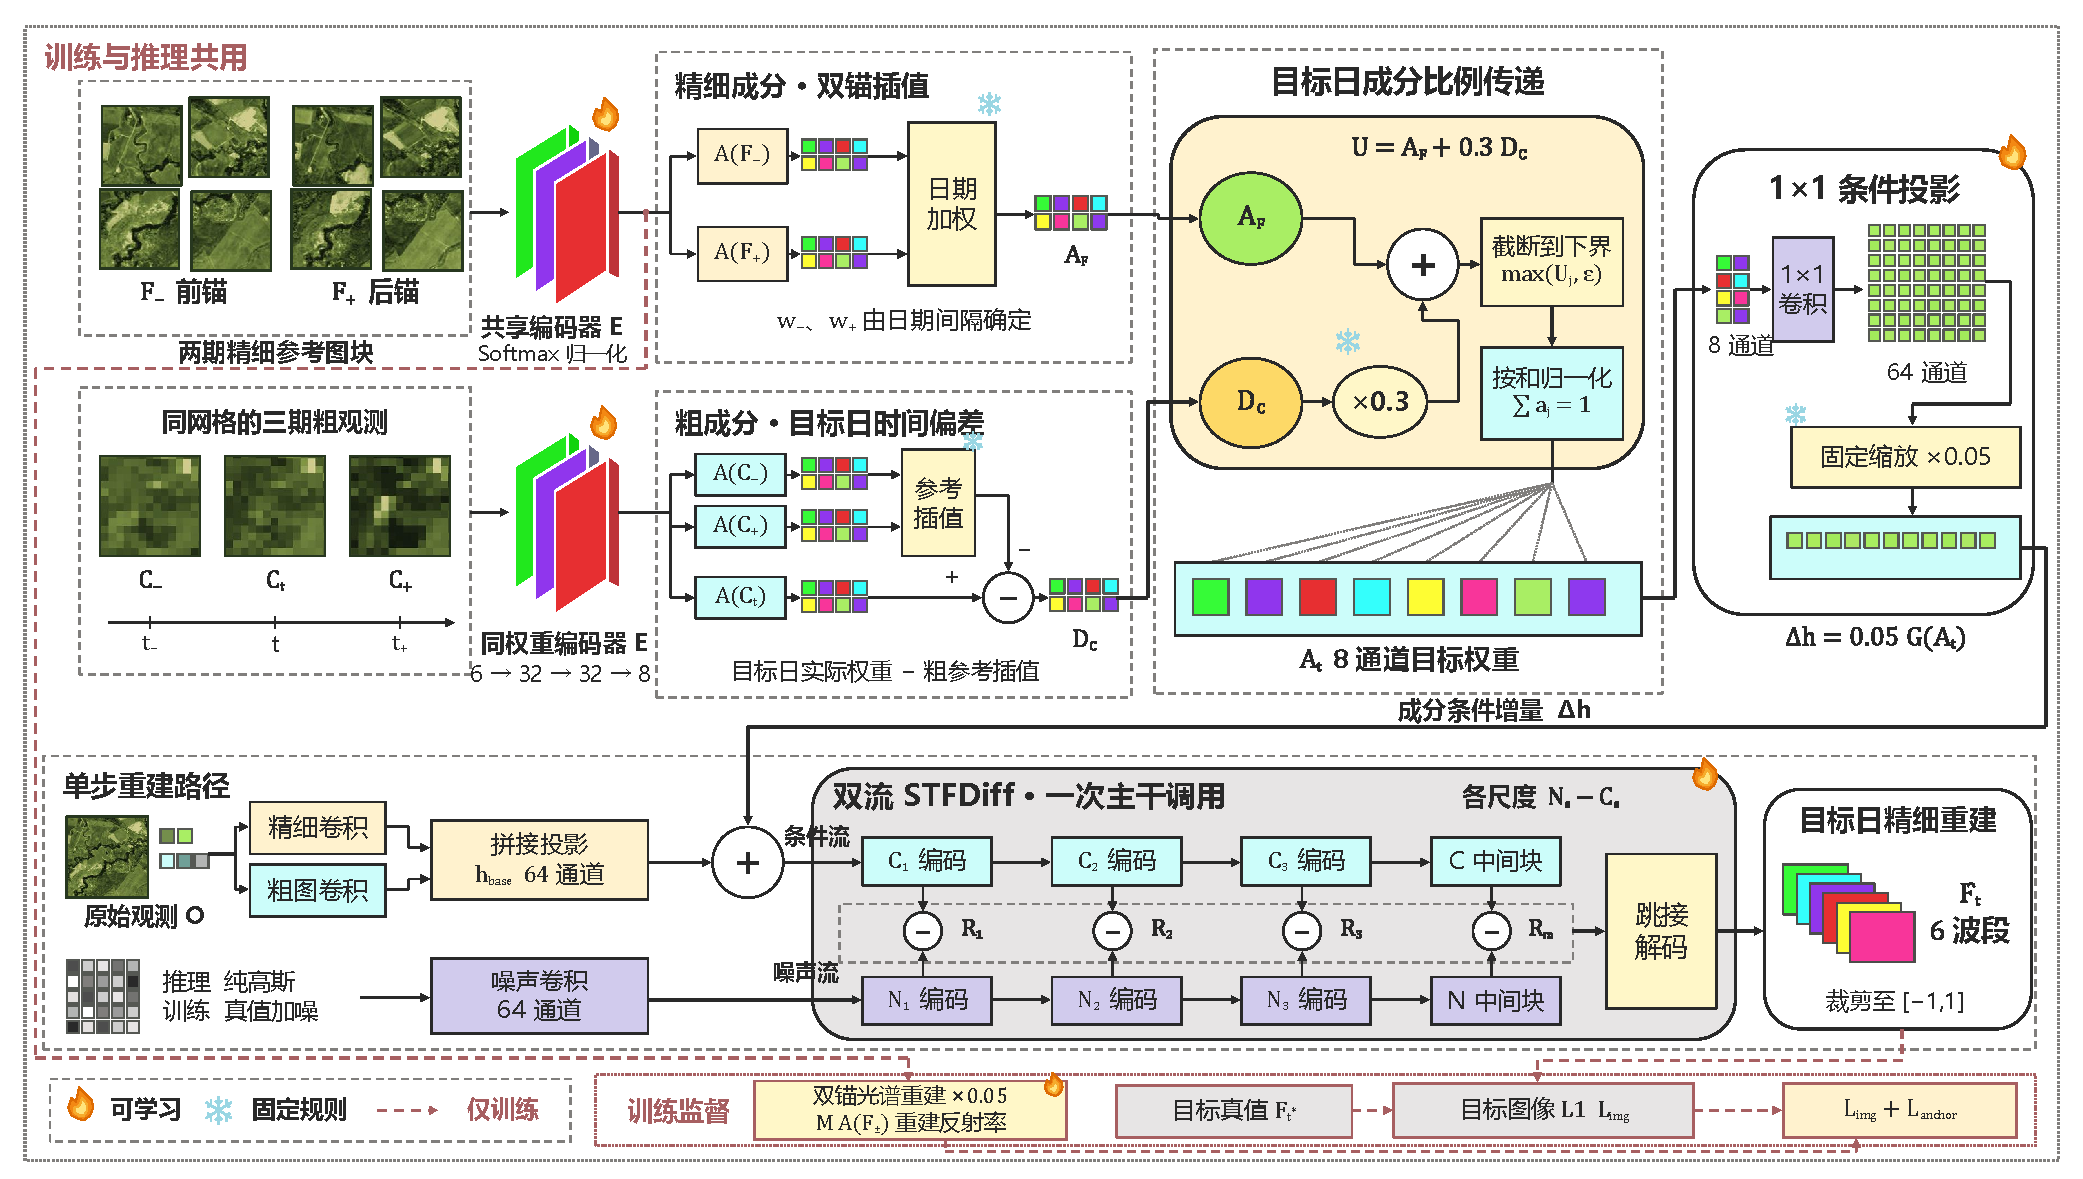
\includegraphics[width=\textwidth]{mechanism_zh.pdf}
\caption{双锚成分权重修正与单步重建。左上为同一 LGC 图块的五幅可见观测。共享编码器产生八通道权重，目标粗权重相对日期插值的偏差修正精细权重。右侧投影的 $0.05G(A_t)$ 加入原条件流。重建只调用一次主干。火苗标记可学习模块，雪花标记固定规则，红色虚线标记训练监督路径。}
\label{fig:mechanism}
\end{figure*}

\section{引言}
Landsat 等精细分辨率观测能描绘地表边界，但目标日的精细影像往往缺失。MODIS 等粗观测的重访更频繁，可以补充目标日观测。双锚时空融合用目标日前后的精细影像、对应的粗影像以及目标日粗影像重建目标日精细反射率。洪水、植被变化等事件可能改变参考影像中的结构，而粗像元中的空间混合会削弱变化位置的可辨识性。

STFDiff 用历史观测对精细影像的生成去噪过程施加条件~\citep{huang2024stfdiff}。采用单次主干调用时，输入条件需要在有限推理预算下提供结构与时间线索。本文考察在原始条件之外显式编码目标日时间偏差能否改善重建。我们将日期加权的精细参考作为出发点，在共享的潜在权重空间传递粗观测偏差，再将结果投影至原条件入口。这样可以在配对的主干和调用次数下比较这条新增路径。

本文同时记录验证集选出的最佳权重和统一的第 40 轮结果，分析 I10 在完整变体集合中的表现。配对块误差、目标权重熵和固定检查点干预用于核对重建改善与时间修正是否对应。本文的实测范围为同一 LGC 开发日期。

\section{相关工作}
STARFM 和 FSDAF 利用可用观测估计时空变化。FSDAF 用光谱解混与薄板样条分配粗尺度残差~\citep{gao2006starfm,zhu2016fsdaf}。STFDiff 则通过条件扩散学习精细影像分布~\citep{huang2024stfdiff}。SA-STF 在残差扩散中引入时序特征对齐和语义自适应融合，并指出缺少匹配参考的罕见突变仍限制细节恢复~\citep{zhang2026sastf}。WPFM-STF 从学习的时空先验出发，以小波细节约束辅助少步流匹配~\citep{hu2026wpfm}。其局部案例显示，全块辐射偏差降低后，细尺度空间误差仍可能保留。

EndNet 等高光谱模型以非负基和成分表示生成光谱~\citep{ozkan2019endnet}。I10 用共享的八通道表示连接粗细观测和不同日期。成分基监督两个精细参考的辅助重建，目标日精细影像由单步骨干输出。成分通道的物理含义需要独立证据。

\section{方法}
\subsection{观测与单步基线}
记较早和较晚的精细参考为 $F_-$ 和 $F_+$，相应粗观测为 $C_-$ 和 $C_+$，目标日粗观测为 $C_t$。时间间隔 $\Delta_-=t-t_-$ 和 $\Delta_+=t_+-t$ 随观测输入。图块大小为 $256\times256$，每幅图含六个波段。反射率先映射到 $[-1,1]$，$\reflectance(X)=(X+1)/2$ 将其还原至 $[0,1]$。

基线以双流骨干分别编码观测条件和带噪状态。条件流对精细参考与粗观测分别做卷积编码，再拼接投影为 $64$ 通道的 $h_{\mathrm{base}}$。各尺度的噪声流减去对应的条件流特征，残差通过跳接进入解码器。主干以噪声级别为条件，输出目标日预测 $\widehat F_t$。

\subsection{双锚成分权重修正}
共享编码器 $E$ 依次采用 $3\times3$ 卷积、$3\times3$ 逐通道卷积和 $1\times1$ 投影，通道数为 $6,32,32,8$。在位置 $p$ 对通道做 softmax，得到
\begin{equation}
 A(X,p)=\operatorname{softmax}_{j}\!\left[E(\reflectance(X))(p)\right].
 \label{eq:weights}
\end{equation}
五幅图的权重共享这一编码器。记 $w_+=\Delta_-/(\Delta_-+\Delta_+)$ 和 $w_-=1-w_+$。省略位置索引，构造精细参考插值 $A_F$ 与目标粗偏差 $D_C$。
\begin{align}
 A_F &= w_-A(F_-)+w_+A(F_+),\\
 D_C &= A(C_t)-w_-A(C_-)-w_+A(C_+).
 \label{eq:coarse}
\end{align}
粗偏差在同一潜在空间内改变精细参考权重。逐通道将下界设为 $10^{-6}$，再按通道和归一化。
\begin{align}
 U&=A_F+0.3D_C,\\
 V_j&=\max(U_j,10^{-6}),\qquad
 A_{t,j}=\frac{V_j}{\sum_{\ell=1}^8 V_\ell}.
 \label{eq:transfer}
\end{align}
学习的 $1\times1$ 投影 $G$ 把八通道权重映射为 $64$ 通道。I10 将 $h_{\mathrm{base}}$ 替换为 $h_{\mathrm{base}}+0.05G(A_t)$。其余输入与基线共用，信息流见图~\ref{fig:mechanism}。

\subsection{训练监督与推理}
训练使用 100 级余弦噪声调度~\citep{nichol2021improved}。取噪声索引 $k$，根据目标真值 $\target$ 和标准高斯噪声 $\varepsilon$ 构造
\begin{equation}
 X_k=\sqrt{\bar\alpha_k}\target+\sqrt{1-\bar\alpha_k}\varepsilon.
\end{equation}
目标日预测裁剪至 $[-1,1]$。训练中还以共享基 $M=\operatorname{sigmoid}(\Theta)$ 重建精细参考，$\Theta\in\mathbb R^{6\times8}$。总损失为
\begin{align}
 \mathcal L={}&\avg{|\widehat F_t-\target|}\\
 &+0.05\sum_{i\in\{-,+\}}
  \avg{|M A(F_i)-\reflectance(F_i)|}.
 \label{eq:objective}
\end{align}
尖括号表示对波段与空间求均值。推理从标准高斯噪声出发，以 $k=99$ 调用一次主干并返回裁剪后的预测。基线和 I10 都使用一次去噪调用，I10 另增加 \ExtraParameters{} 个参数和条件编码计算。基线共有 \BaseParameters{} 个参数。

\begin{table*}[!t]
\centering
\caption{同一 LGC 开发划分上三十组从零复验的平均块 RMSE。每种子各 15 组。最佳值来自各组最小验证 RMSE 检查点，共同终点为第 40 轮。}
\label{tab:main}
\small
\setlength{\tabcolsep}{12pt}
\begin{tabular}{lrrrr}
\toprule
& \multicolumn{2}{c}{种子 42} & \multicolumn{2}{c}{种子 123}\\
\cmidrule(lr){2-3}\cmidrule(lr){4-5}
方法 & 最佳检查点 & 第 40 轮 & 最佳检查点 & 第 40 轮\\
\midrule
\PrimaryRows
\bottomrule
\end{tabular}
\end{table*}

\begin{figure*}[!t]
\centering
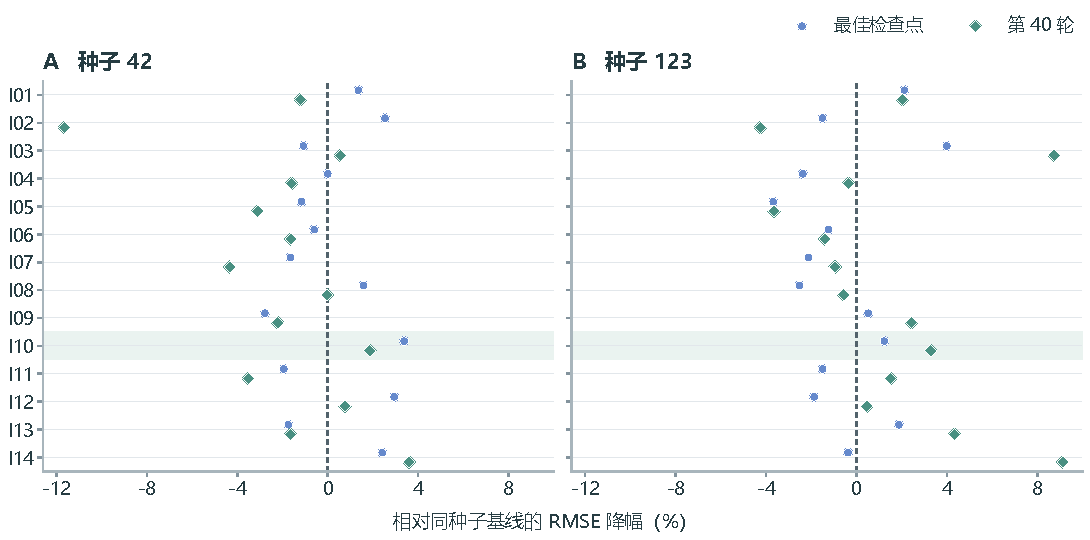
\includegraphics[width=.94\textwidth]{gains_zh.pdf}
\caption{相对同种子基线的 RMSE 降幅。圆点来自各自最佳检查点，菱形来自共同第 40 轮。正值为误差下降，负值为误差升高。}
\label{fig:gains}
\end{figure*}

\section{实验协议}
\subsection{数据、配对与指标}
LGC Landsat--MODIS 地表反射率序列由 CSIRO 发布~\citep{emelyanova2013blending,csiro2014lgc}。冻结训练划分含 10 个三元组的 1,200 块，开发验证含 120 个互不重叠的块，目标日为 2005 年 3 月 2 日。粗数据已配准至共同网格。训练三元组的日期与验证目标日分离。该开发日期曾用于项目探索。

六轮初筛使用同一旧权重微调，比较基线和十四个变体。随后两种子（42、123）各执行基线加十四个变体的 40 轮从零训练。种子内配对共享主干初始化、样本次序和基础噪声。复验采用 Adam，峰值学习率 $2\times10^{-4}$，梯度累积为 2，每轮 600 个优化器更新。各组共用划分和选模规则。

验证对每块使用三个固定噪声实现，先求每次重建的反射率 RMSE，再等权平均。主表同时报告最佳验证检查点和共同第 40 轮。SSIM、光谱角（SAM，弧度）、ERGAS 和相关系数（CC）由最佳 RMSE 权重导出。

\subsection{块级配对与干预}
最佳权重的逐块比较先对三个噪声实现平均，再求同种子基线减 I10 的误差差值。将验证网格按 $2\times2$ 图块分成 30 个空间块，进行 10,000 次有放回重采样，报告 $2.5$ 和 $97.5$ 百分位。区间描述当日场景内的空间变异。另按 $C_t$ 相对粗参考日期插值的平均绝对偏离度排序，每个三分位包含 40 块。

固定权重干预使用 seed 42 的第 32 轮检查点、两块验证样本和每块同一个噪声。比较原始 I10、置零 $D_C$、在块内置乱 $32\times32$ 子块，以及移除完整的成分条件增量。受控推理用于检验已训权重的响应。

\begin{figure*}[!t]
\centering
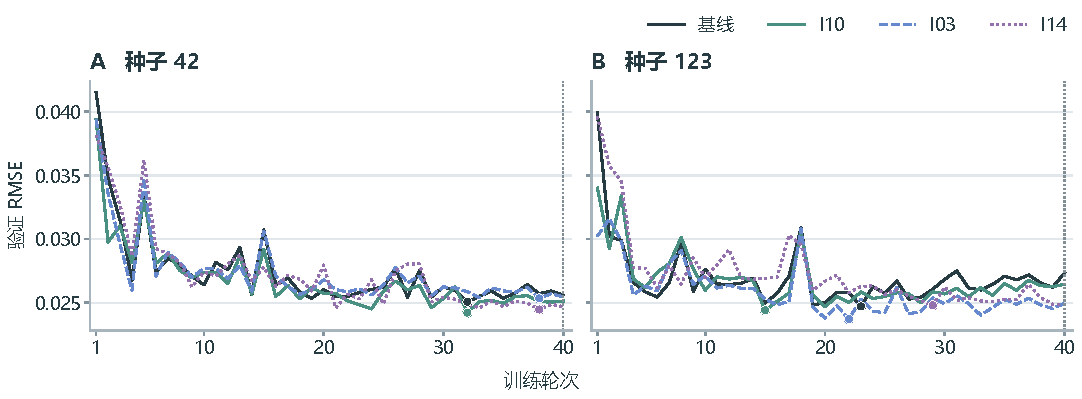
\includegraphics[width=.94\textwidth]{trajectory_zh.pdf}
\caption{基线和代表性变体的验证轨迹。标记为各曲线的最佳轮，竖点线为共同的第 40 轮。全部逐轮数据随实验档案提供。}
\label{fig:trajectory}
\end{figure*}

\begin{figure*}[!t]
\centering
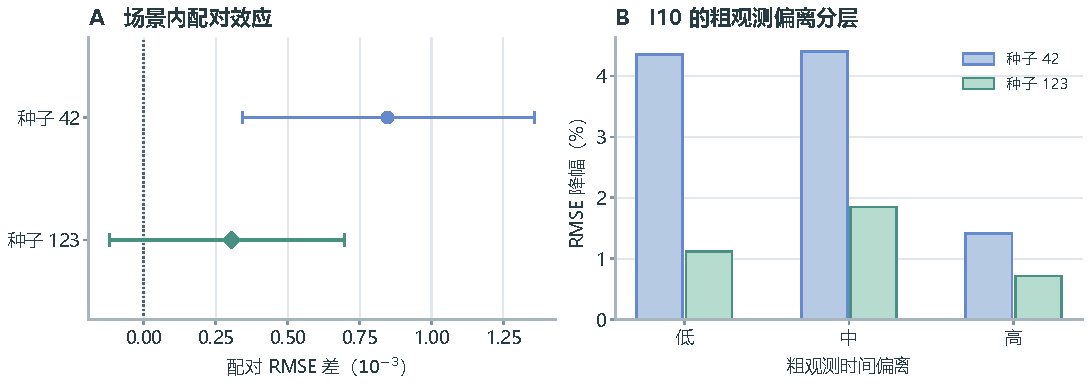
\includegraphics[width=.94\textwidth]{diagnostics_zh.pdf}
\caption{I10 的最佳检查点诊断。A 以基线减 I10 计算配对平均 RMSE 差，区间来自场景内空间块重采样。B 对 120 个块按粗观测时间偏离分成三等份，报告相对该分组内基线的均值降幅。}
\label{fig:diagnostics}
\end{figure*}

\section{结果}
\subsection{随种子与检查点变化的排序}
六轮初筛中，十四个变体的最佳 RMSE 均高于原始权重的参照值 \ScreenReference{}。从零复验后，各变体的相对排序发生变化。表~\ref{tab:main} 和图~\ref{fig:gains} 保留了全部比较。

I10 的最佳 RMSE 在 seed 42 从 \BaseBestA{} 降至 \MainBestA{}，在 seed 123 从 \BaseBestB{} 降至 \MainBestB{}。共同第 40 轮分别从 \BaseFinalA{} 降至 \MainFinalA{}、从 \BaseFinalB{} 降至 \MainFinalB{}。I01 在两个种子的最佳检查点均有改善，seed 42 的第 40 轮误差升高。I03、I12 和 I14 在两个种子的第 40 轮均改善，至少一个种子的最佳检查点相对基线退化。I14 取得两个种子最低的第 40 轮 RMSE。I03 取得 seed 123 的最低最佳检查点 RMSE。图~\ref{fig:trajectory} 将这些差异放在训练轨迹中呈现。

\begin{table}[!t]
\centering
\caption{基线与 I10 的最佳检查点的次要指标。SAM 以弧度计。}
\label{tab:secondary}
\small
\setlength{\tabcolsep}{2.7pt}
\begin{tabular}{rlrrrrr}
\toprule
种子 & 方法 & 最佳轮 & SSIM $\uparrow$ & SAM $\downarrow$ & ERGAS $\downarrow$ & CC $\uparrow$\\
\midrule
\SecondaryRows
\bottomrule
\end{tabular}
\end{table}

\subsection{光谱指标和空间分布}
表~\ref{tab:secondary} 显示，I10 的 SAM 和 ERGAS 在两种子均降低。两种子的 CC 均略降，SSIM 分别小幅下降和上升。光谱指标与整体 RMSE 的改善同时出现，结构指标呈现混合变化。

在最佳检查点，I10 的逐块平均差为 \MeanPairA{} 和 \MeanPairB{}（$10^{-3}$），有 \BetterPatchesA{} 和 \BetterPatchesB{} 个块改善。seed 42 场景内空间重采样区间为 $[\LowPairA,\HighPairA]\times10^{-3}$。seed 123 的区间为 $[\LowPairB,\HighPairB]\times10^{-3}$，跨越零（图~\ref{fig:diagnostics}A）。按可见粗偏离分层后，两种子在三个分位组的平均 RMSE 均下降。高偏离组的降幅在各自种子内最小（图~\ref{fig:diagnostics}B）。分层衡量相对粗参考插值的偏离，地表类型和真实细尺度变化仍需专门的标注与检测。

\subsection{潜在权重与粗偏差响应}
两个 I10 检查点的逐块像素平均熵中位数均约为 $1.037\times10^{-4}$ nat，接近单通道权重经式~\eqref{eq:transfer} 截断并归一化后的值。权重高度集中，适合先从占优通道和投影幅度检验其作用。

在两块干预样本上，完整 I10 的 RMSE 为 \ProbeFull{}。置零和置乱 $D_C$ 后分别为 \ProbeZero{} 与 \ProbeShuffle{}。移除整条注入后为 \ProbeNoInjection{}，基线为 \ProbeBase{}。这两块对整条注入和其中的目标日粗偏差表现出不同的敏感性。对完整验证场景的响应及重新训练后的归因仍需验证。

\section{讨论}
两个种子的配对结果支持在下一阶段保留 I10，并将 I03 和 I14 的端点表现作为有价值的对照。全组结果显示，比较所用的检查点规则改变了对各变体的判断。I10 在共同终点和验证选模两种规则下都降低误差，使该原型值得进一步检查。空间重采样区间和探针结果说明，这一观察有明确的场景与机制解释边界。

两个种子均出现的权重集中和小样本中近零的粗偏差响应，提示条件增量的收益未能直接归因于时变成分传递。下一步应在全量块上冻结权重做去除和置乱，并用无粗偏差、可学习常量条件及等容量原始反射率残差支路配对重训。该比较可以检验目标日位置和时间信息在现有骨干中有多少独立贡献。

外部主比较需复现同样使用五幅观测的强方法，在共同训练划分和相同评价规则下配对比较原版与改造版。SA-STF 的补充材料列出的训练日期包含当前开发目标日，复用作者权重时须按训练暴露限定用途~\citep{zhang2026sastf}。独立日期和跨区测试应在模型选择冻结后执行，并同时测细尺度变化错定位、稳定区误报和推理开销。

\section{结论}
在同一开发日期的三十组复验中，I10 在两个种子的最佳检查点与共同第 40 轮均降低单步 STFDiff 的验证 RMSE。权重集中及小样本干预将下一步工作指向时间修正的归因。独立日期上的变化恢复和同协议外部较强基线比较，是确认这一方法价值的后续实验。

\section*{代码与实验记录}
归档包含六轮初筛和两种子复验的运行配置、逐轮日志、逐块指标、源码快照、权重和续训点，以及本文的图表复算脚本。\href{https://github.com/qing1989620/paper-shikongyaogan/releases/tag/stf-stage-20261125}{GitHub 发布档案与校验码}

\FloatBarrier
\balance
\bibliographystyle{IEEEbib}
\bibliography{refs}
\end{document}
